\section{Exploring The Z-Profile}
\label{ch:ExploringZProfile}

\begin{frame}
	\frametitle{Bunch Profile Flavors}
	In searching for absolute convergence between the data and simulation, we have to cross-check several parts of the simulation.
	\begin{itemize}
			\item How does the z-profile effect the data?
			\item Are edge effects important to the final ZDC zvertex distribution?
			\item Once we choose a z-profile, are these z-profiles colliding centrally?
			\item How do bunches collide at the IR?
	\end{itemize}
  \textbf{How Do We Test?}
	\begin{itemize}
			\item Define a metric for convergence
			\item Generate a "perfectly" converged ZDC zvertex distriubtion.
			\item Observe the distribution's shape for maximally overlapped beams
	\end{itemize}
	\textbf{Why Test Different Profiles?}
	\begin{itemize}
		\item Because results for max-overlap looks fishy for various different profiles.
		\item Work is proceeding in parallel between convergence methods + getting the right behavior out of the profile.
	\end{itemize}
\end{frame}

\begin{frame}
\frametitle{Profile Flavors}
\begin{itemize}
  \item Baseline Profile: Amaresh (probably not representative of real beam profile)
	\item Pure Gaussian Profile: Based on overall shape of WCM distribution (probably not representative of real beam profile)
	\item Data-Direct: Exact averaged shape of WCM profile, may be subject to edge effects, lookup error
	\item Fitted Data-Direct: multi-gaussian fit of central profile region, edge effects ignored
\end{itemize}
\end{frame}

\begin{frame}
\frametitle{Collision Geometry}
\begin{figure}
\begin{center}
	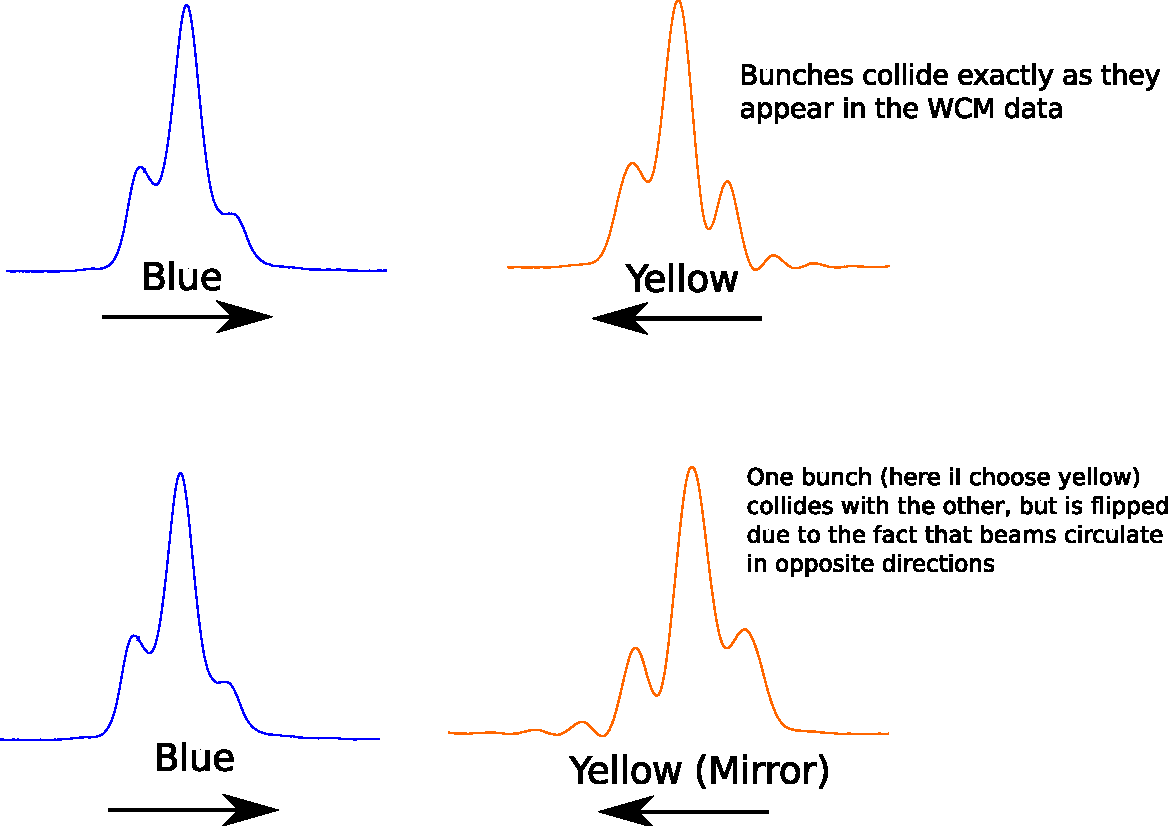
\includegraphics[width=0.6\linewidth]{../ExploringZProfile/figs/normal_vs_mirrored.pdf}
\end{center}
\caption{ I discussed with Angelika which way bunches should collide, since WCM
data shows that bunches are asymmetric. Angelika says they collide such that the
two bunches overlap maximally. (I.e.: they collide "normal" not "mirrored")}
\label{fig:bunchcollisiondirection}
\end{figure}
\end{frame}

\begin{frame}{New Bunch Alignment}
\begin{figure}
\begin{center}
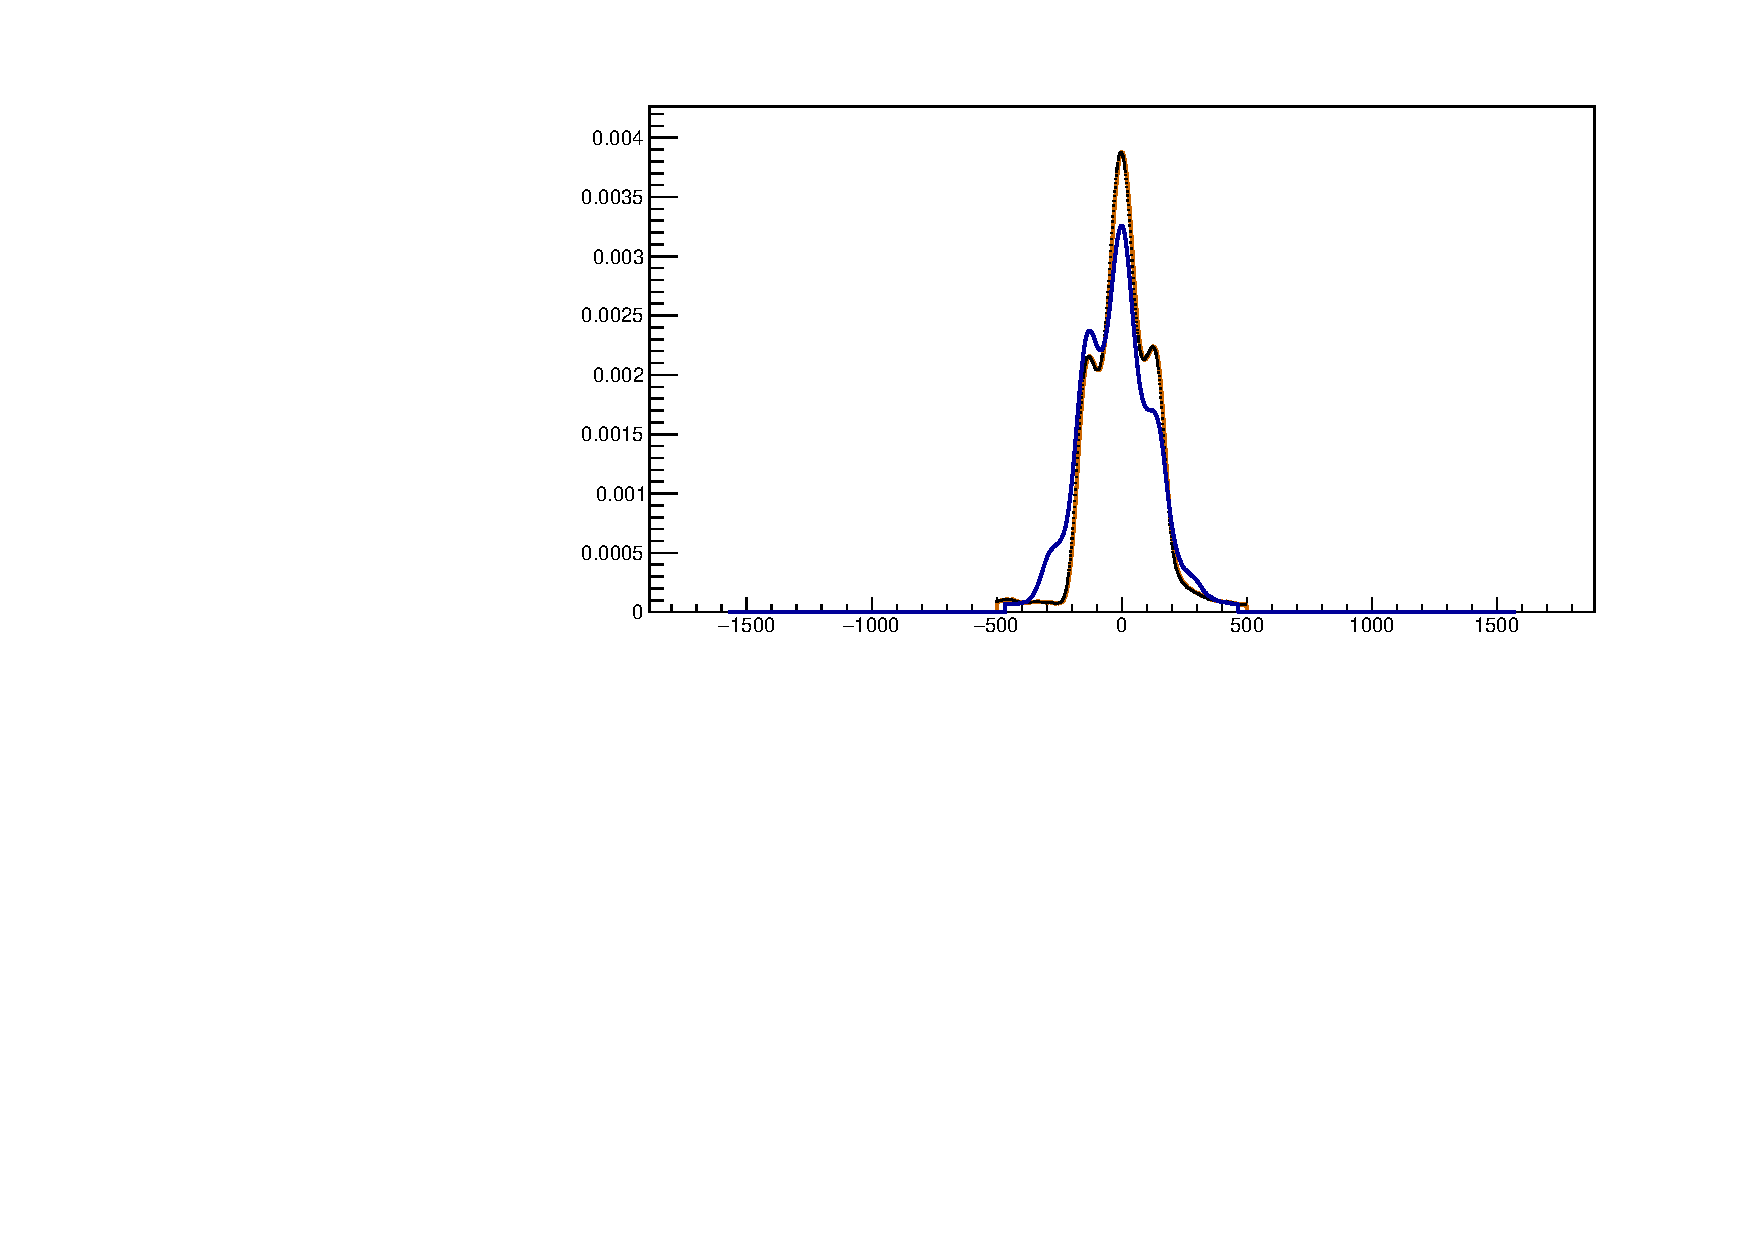
\includegraphics[width=0.8\linewidth]{../ExploringZProfile/figs/359711_bunch_alignment.pdf}
\end{center}
\caption{Bunches have been aligned such that they line up at their maxima,
rather than lining up according to a time window. We define the time binning such
that at arbitrary time t = 0, these maxima overlap.}
\label{fig:359711_bunch_alignment}
\end{figure}
\end{frame}

\begin{frame}{Lookup Accuracy}
\begin{figure}
\begin{center}
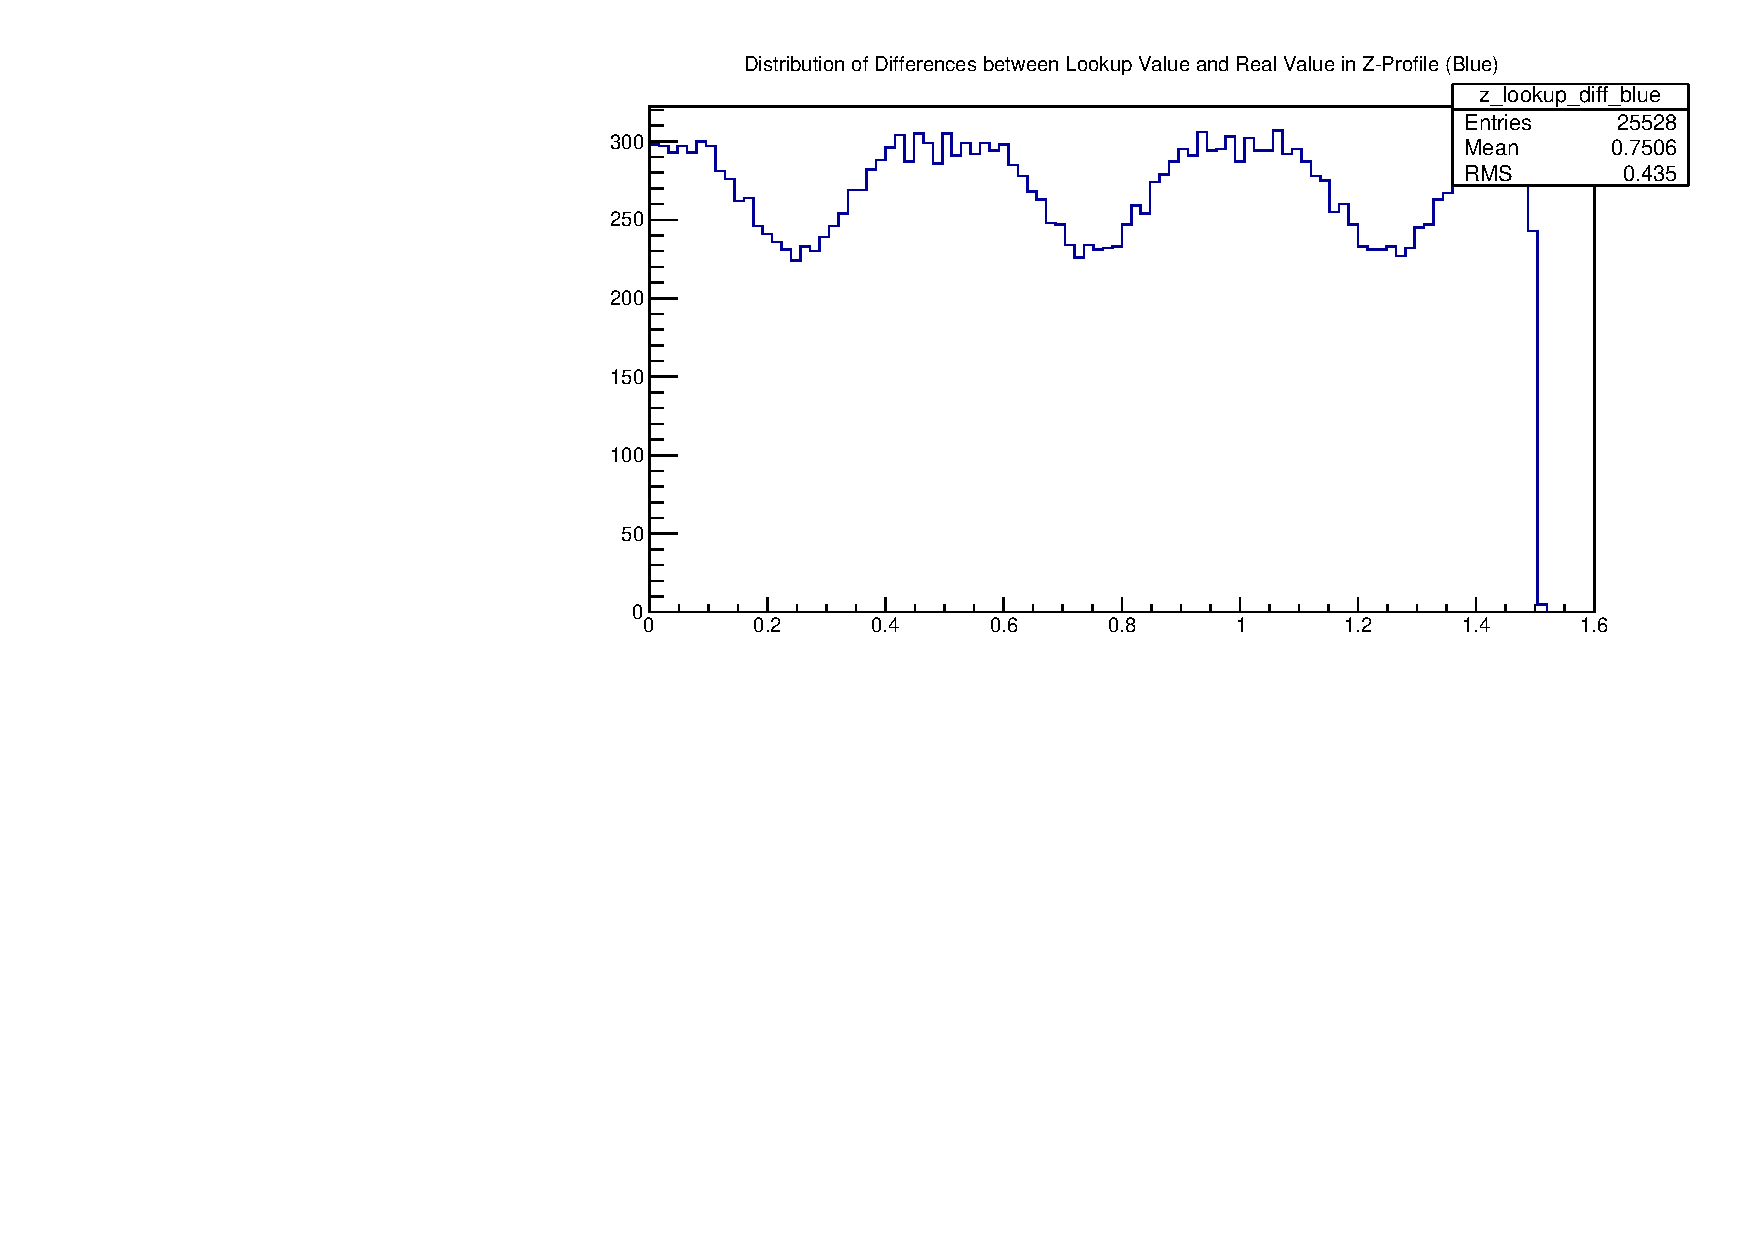
\includegraphics[width=0.8\linewidth]{../ExploringZProfile/figs/359711_lookup_z.pdf}
\end{center}
\caption{Instead of interpolation between defined profile points, we instead bin
time finely, which results in a spatial binning of 1.5 cm in z. Pictured here
is a histogram, binned in z, where we fill it with the difference between the
looked up z value, and the z-value desired. The yellow beam lookup calls are
identical.}
\label{fig:359711_lookup_z}
\end{figure}
\end{frame}

\begin{frame}{Resulting ZDC Z-Profile}
\begin{figure}
\begin{center}
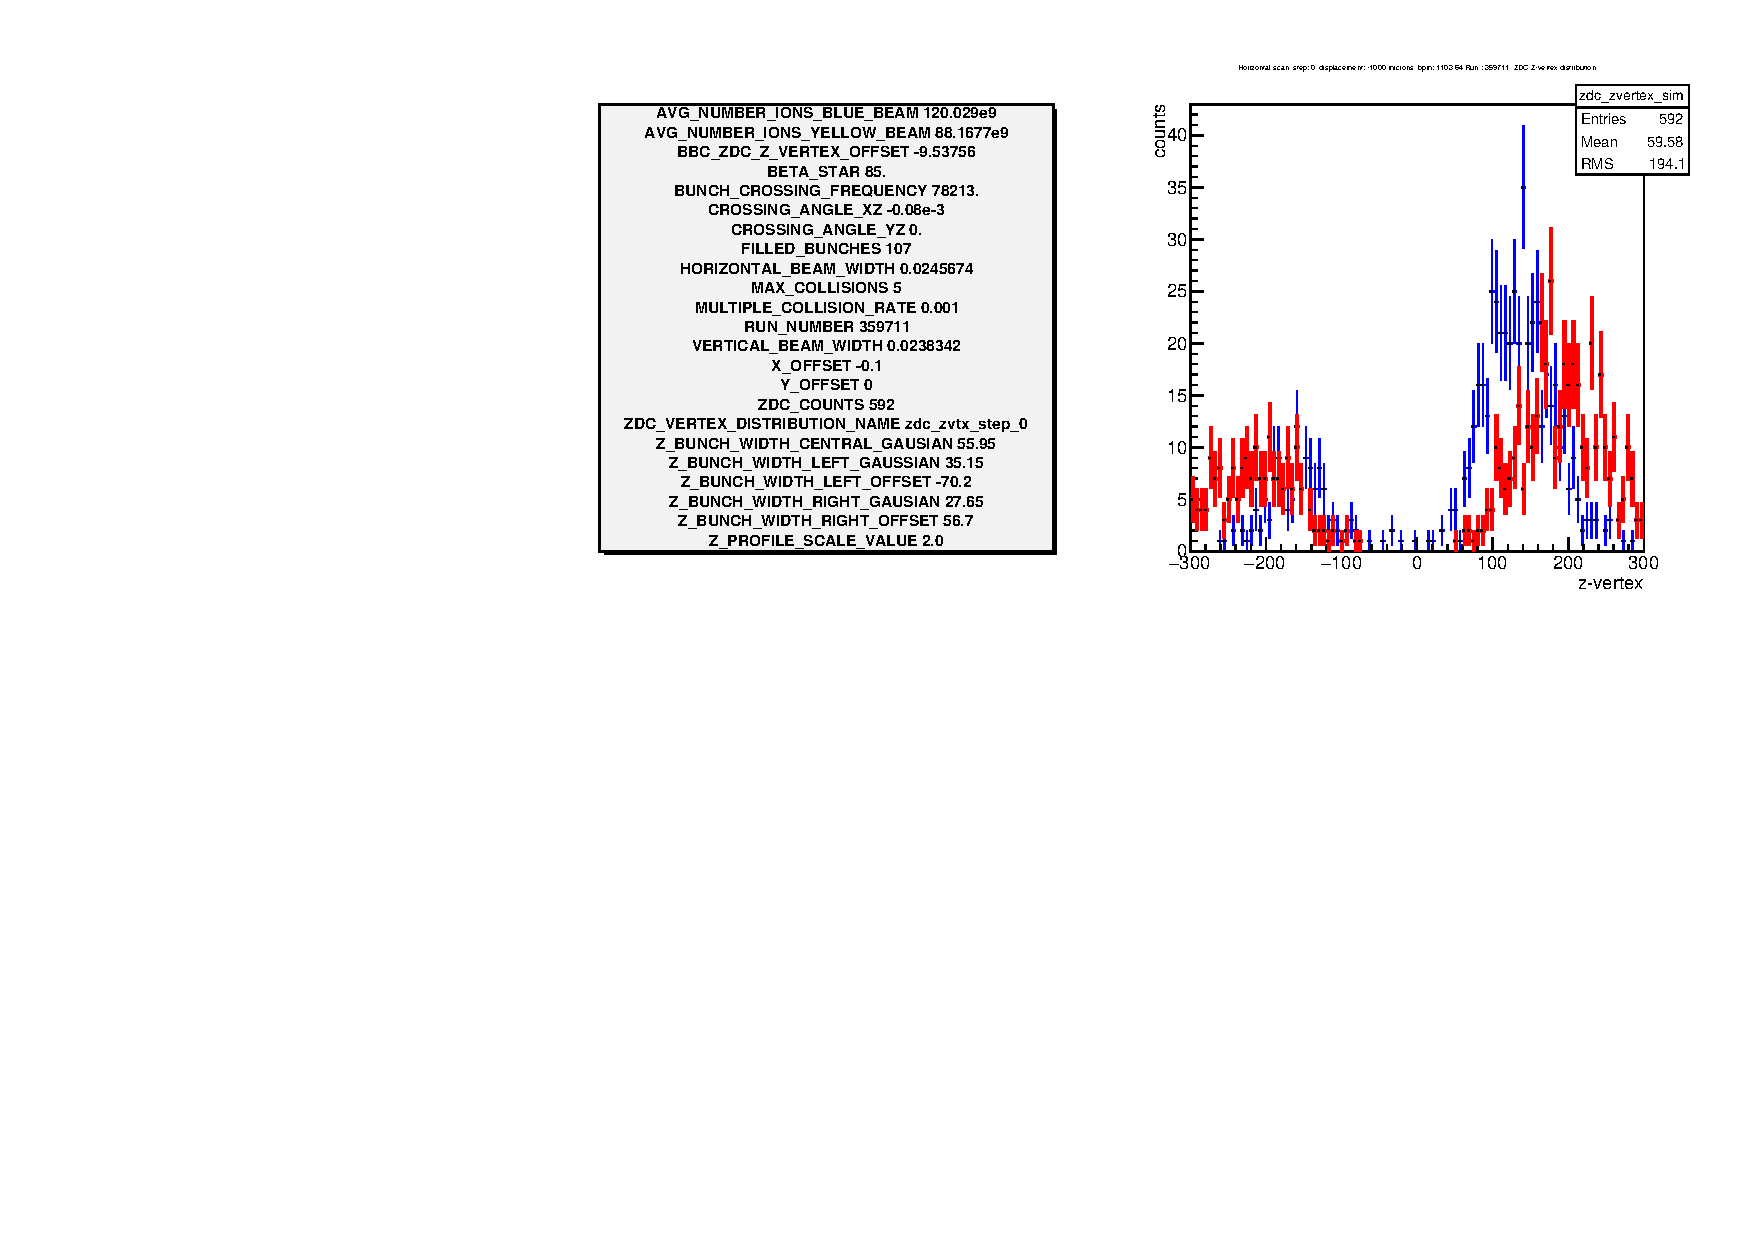
\includegraphics[width=0.8\linewidth]{../ExploringZProfile/figs/359711_step_0_zvertex_compare.pdf}
\end{center}
\caption{We get slightly better results by adjusting the interaction between
bunches to overlap at z = 0, but the distribution is still not well aligned. The
peaks seem to be separated too much.}
\label{fig:359711_step_0_zvertex_compare}
\end{figure}
\end{frame}

\begin{frame}{Resulting ZDC Z-Profile - With Hand Tuning}
\begin{figure}
\begin{center}
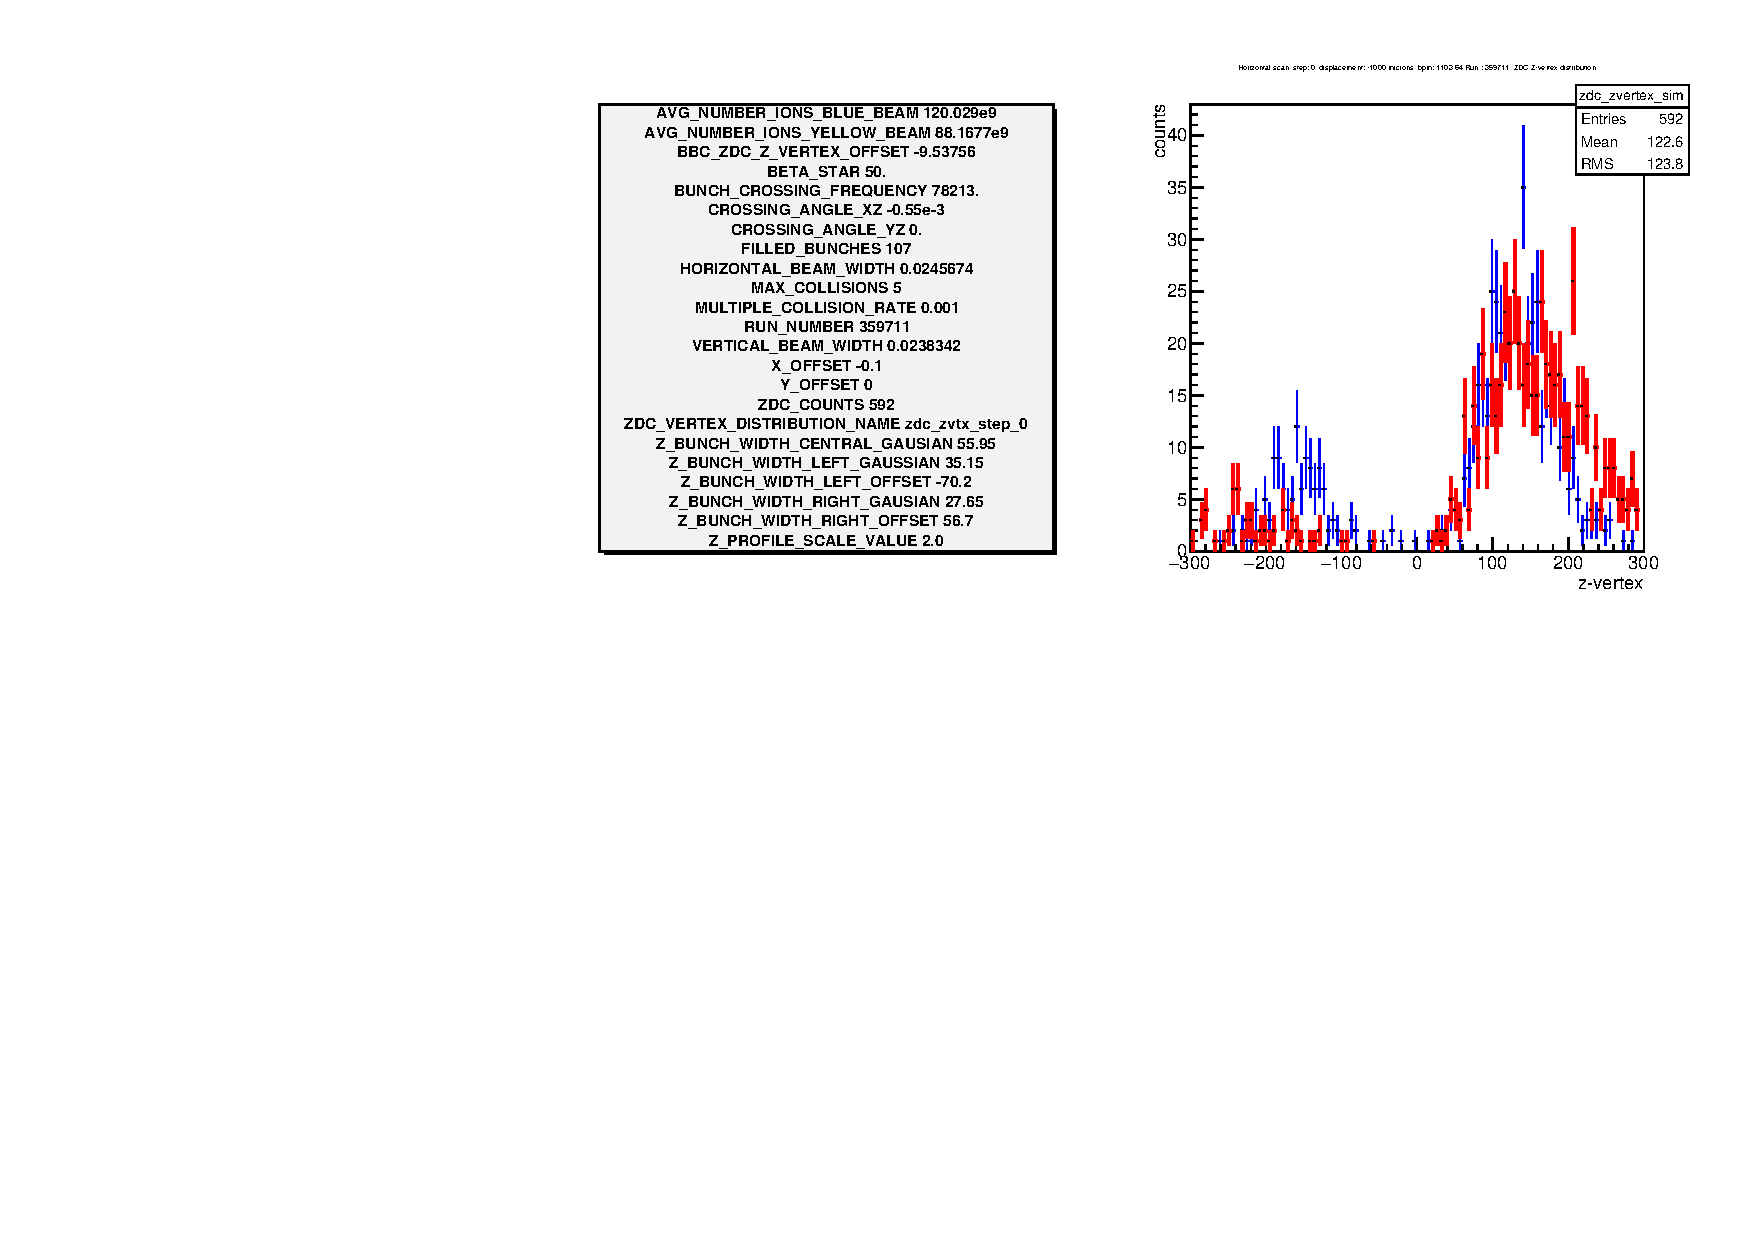
\includegraphics[width=0.8\linewidth]{../ExploringZProfile/figs/359711_step_0_zvertex_compare_tuned.pdf}
\end{center}
\caption{We get slightly better results by tuning $\theta_{XZ}$ and $\beta^{*}$.
	As expressed in previous weeks, I am concerned that the simulations present a
	fine tuning problem. The distributions seem to exhibit the right sort of
behavior at maximum and minimum overlap.}
\label{fig:359711_step_0_zvertex_compare_tuned}
\end{figure}
\end{frame}

\begin{frame}{Max Overlap ZDC Profile - No Tuning}
\begin{figure}
\begin{center}
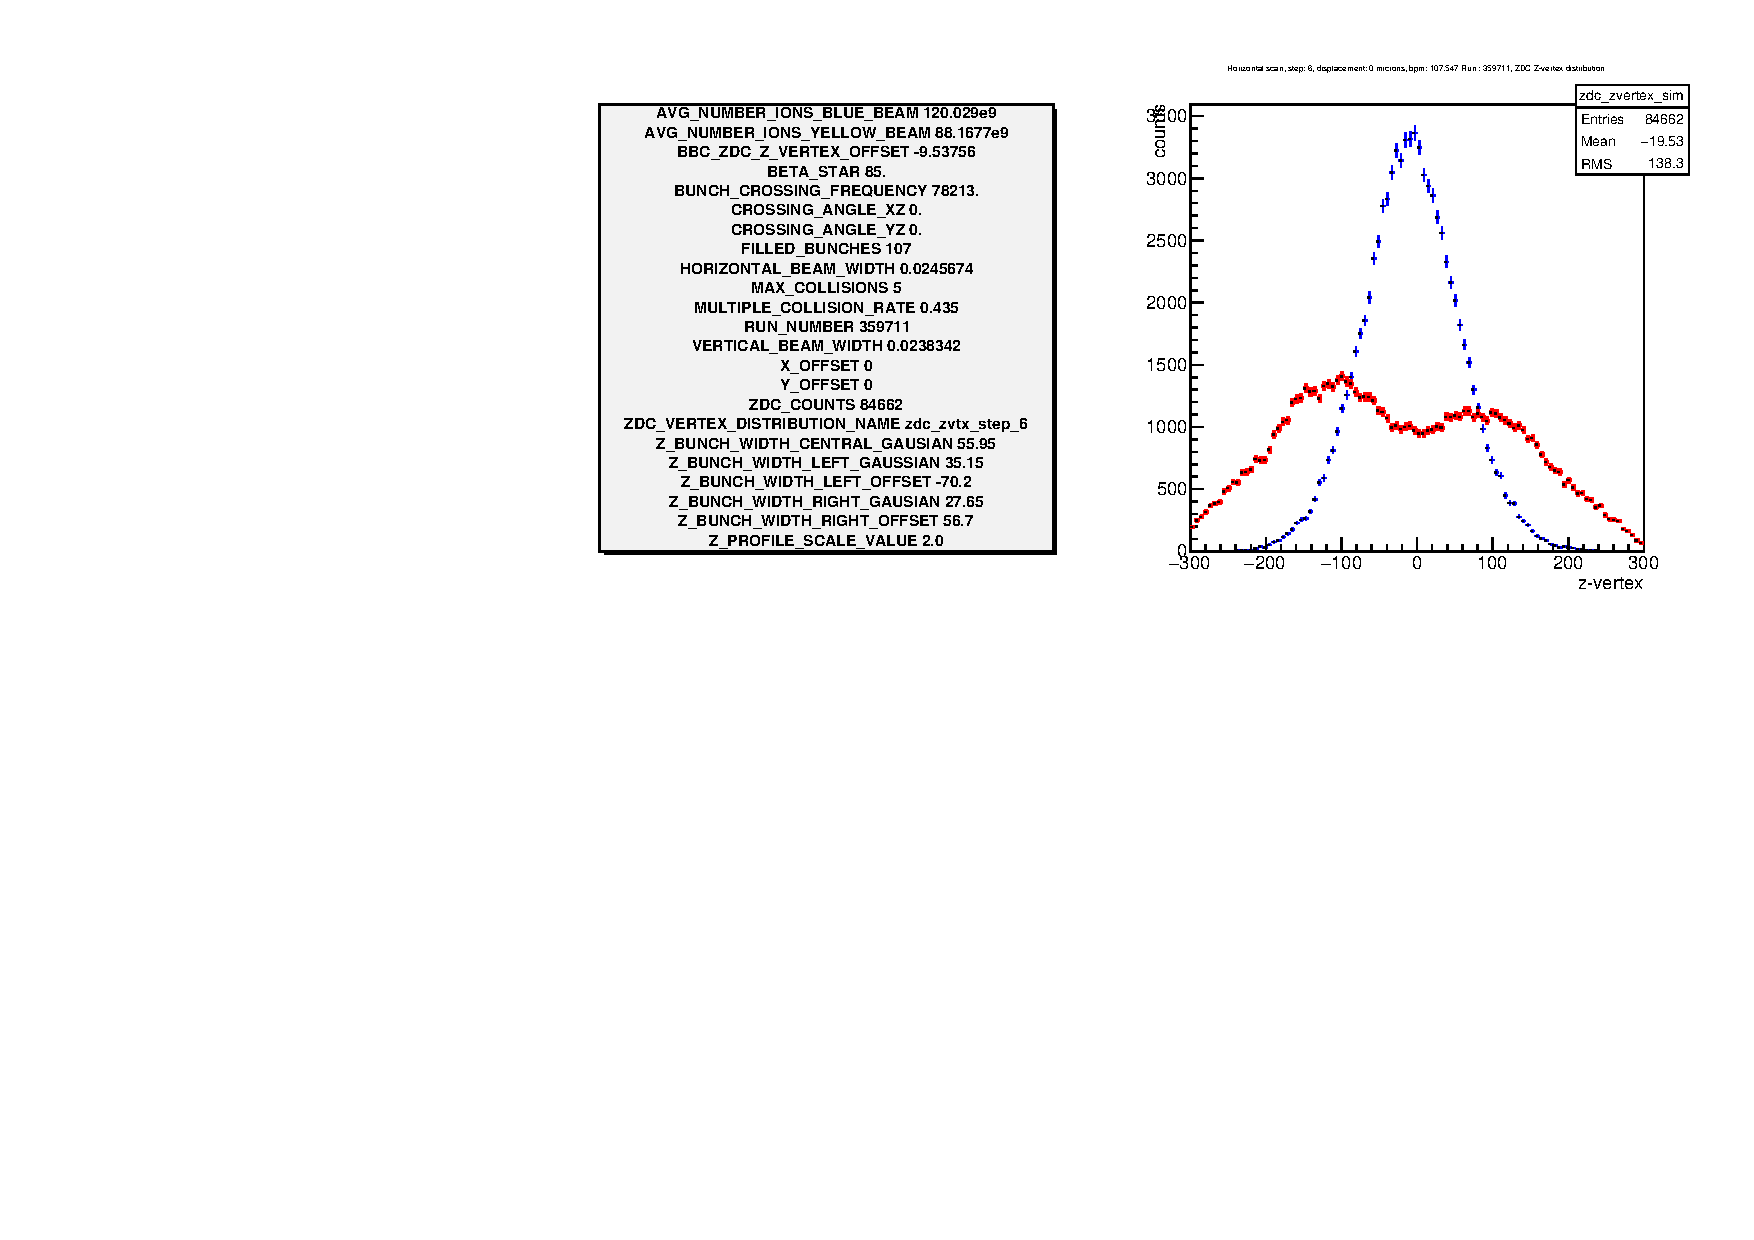
\includegraphics[width=0.8\linewidth]{../ExploringZProfile/figs/359711_step_6_zvertex_compare.pdf}
\end{center}
\caption{
	As a sanity check, we show the max-overlap profile. This plot is generated
	using the best-eye-matching configuration parameters for a different z-vertex
	profile. We will see later, that, even with no displacement, the bunch profile
	shape + presence of a crossing angle can make the max-overlap ZDC vertex
	profile asymmetric.
}
\label{fig:359711_step_6_zvertex_compare}
\end{figure}
\end{frame}


\begin{frame}{Discussion}
	\begin{itemize}
		\item So far, hand tuning with the WCM data profiles has not proven as
			successful as with the originally used profile.
		\item We can pick a z-profile, and a 'well converged' set of parameters, and
			study the effect of the z-profile shape on the ZDC z-vertex distriubtion
		\item While we do this, we can also check to see how beams collide at the
			IR, as Sasha mentioned some time ago that if profiles do not overlap
			correctly, we will generate a funny looking ZDC z-vertex shape.
		\item During these studies, keep in mind:
			\begin{itemize}
					\item Each z-profile may require a different set of "best parameters"
						to look good
					\item To account for possible differences, we show distributions with,
						and without crossing angles.
					\item Split spectra may be due to crossing angle, not offest beam
			\end{itemize}
	\end{itemize}
\end{frame}
